\documentclass[conference]{IEEEtran}
\usepackage{enumerate}
\usepackage{todonotes}
\ifCLASSINFOpdf
  % \usepackage[pdftex]{graphicx}
  % declare the path(s) where your graphic files are
  % \graphicspath{{../pdf/}{../jpeg/}}
  % and their extensions so you won't have to specify these with
  % every instance of \includegraphics
  % \DeclareGraphicsExtensions{.pdf,.jpeg,.png}
\else
  % or other class option (dvipsone, dvipdf, if not using dvips). graphicx
  % will default to the driver specified in the system graphics.cfg if no
  % driver is specified.
  % \usepackage[dvips]{graphicx}
  % declare the path(s) where your graphic files are
  % \graphicspath{{../eps/}}
  % and their extensions so you won't have to specify these with
  % every instance of \includegraphics
  % \DeclareGraphicsExtensions{.eps}
\fi
% graphicx was written by David Carlisle and Sebastian Rahtz. It is
% required if you want graphics, photos, etc. graphicx.sty is already
% installed on most LaTeX systems. The latest version and documentation
% can be obtained at: 
% http://www.ctan.org/pkg/graphicx
% Another good source of documentation is "Using Imported Graphics in
% LaTeX2e" by Keith Reckdahl which can be found at:
% http://www.ctan.org/pkg/epslatex
%
% latex, and pdflatex in dvi mode, support graphics in encapsulated
% postscript (.eps) format. pdflatex in pdf mode supports graphics
% in .pdf, .jpeg, .png and .mps (metapost) formats. Users should ensure
% that all non-photo figures use a vector format (.eps, .pdf, .mps) and
% not a bitmapped formats (.jpeg, .png). The IEEE frowns on bitmapped formats
% which can result in "jaggedy"/blurry rendering of lines and letters as
% well as large increases in file sizes.
%
% You can find documentation about the pdfTeX application at:
% http://www.tug.org/applications/pdftex

% *** SUBFIGURE PACKAGES ***
%\ifCLASSOPTIONcompsoc
%  \usepackage[caption=false,font=normalsize,labelfont=sf,textfont=sf]{subfig}
%\else
%  \usepackage[caption=false,font=footnotesize]{subfig}
%\fi
% subfig.sty, written by Steven Douglas Cochran, is the modern replacement
% for subfigure.sty, the latter of which is no longer maintained and is
% incompatible with some LaTeX packages including fixltx2e. However,
% subfig.sty requires and automatically loads Axel Sommerfeldt's caption.sty
% which will override IEEEtran.cls' handling of captions and this will result
% in non-IEEE style figure/table captions. To prevent this problem, be sure
% and invoke subfig.sty's "caption=false" package option (available since
% subfig.sty version 1.3, 2005/06/28) as this is will preserve IEEEtran.cls
% handling of captions.
% Note that the Computer Society format requires a larger sans serif font
% than the serif footnote size font used in traditional IEEE formatting
% and thus the need to invoke different subfig.sty package options depending
% on whether compsoc mode has been enabled.
%
% The latest version and documentation of subfig.sty can be obtained at:
% http://www.ctan.org/pkg/subfig

\hyphenation{op-tical net-works semi-conduc-tor}
\begin{document}

\title{Utilizando a Fase de Empatia do Design Thinking como Facilitadora na Elicitação dos Requisitos de Privacidade
}


% author names and affiliations
% use a multiple column layout for up to three different
% affiliations
\author{\IEEEauthorblockN{Blind}
\IEEEauthorblockA{School of Electrical and\\Computer Engineering\\
Georgia Institute of Technology\\
Atlanta, Georgia 30332--0250\\
Email: http://www.michaelshell.org/contact.html}
\and
\IEEEauthorblockN{Blind}
\IEEEauthorblockA{Twentieth Century Fox\\
Springfield, USA\\
Email: homer@thesimpsons.com}
\and
\IEEEauthorblockN{Blind \\ and Blind}
\IEEEauthorblockA{Starfleet Academy\\
San Francisco, California 96678--2391\\
Telephone: (800) 555--1212\\
}}
% of the page, use this alternative format:
% 
%\author{\IEEEauthorblockN{Michael Shell\IEEEauthorrefmark{1},
%Homer Simpson\IEEEauthorrefmark{2},
%James Kirk\IEEEauthorrefmark{3}, 
%Montgomery Scott\IEEEauthorrefmark{3} and
%Eldon Tyrell\IEEEauthorrefmark{4}}
%\IEEEauthorblockA{\IEEEauthorrefmark{1}School of Electrical and Computer Engineering\\
%Georgia Institute of Technology,
%Atlanta, Georgia 30332--0250\\ Email: see http://www.michaelshell.org/contact.html}
%\IEEEauthorblockA{\IEEEauthorrefmark{2}Twentieth Century Fox, Springfield, USA\\
%Email: homer@thesimpsons.com}
%\IEEEauthorblockA{\IEEEauthorrefmark{3}Starfleet Academy, San Francisco, California 96678-2391\\
%Telephone: (800) 555--1212, Fax: (888) 555--1212}
%\IEEEauthorblockA{\IEEEauthorrefmark{4}Tyrell Inc., 123 Replicant Street, Los Angeles, California 90210--4321}}
\maketitle

\begin{abstract}
The abstract goes here.
\end{abstract}
\IEEEpeerreviewmaketitle

\section{Introduction}

A elicitação de requisitos é uma etapa fundamental no processo de desenvolvimento de software, uma vez que é nesta etapa que o software começa a ser projetado. Alguns problemas relacionados ao insucesso de projetos de desenvolvimento de software são decorrentes de uma elicitação de requisitos incompleta, resultando em sistemas que não compreendem todas as funcionalidades necessárias ou que não incorporam inovações. Apesar dos recursos disponíveis na literatura pela Engenharia de Requisitos, situações como o mercado crescente de
sistemas e a necessidade de inovação aumentam ainda mais a importância de se entender as necessidades e diferenciais dos sistemas, conforme o que os usuários solicitam. Assim, existe uma possibilidade de buscar outras formas de elicitação e uma delas é a utilização de técnicas sugeridas pelo Design Thinking.

A utilização de técnicas de Design Thinking na elicitação de requisitos tem sido bastante utilizadas. Técnicas de Empatia podem ajudar a mapear as necessidades do usuário de maneira mais clara e rápida.



\todo[inline]{Introduzir o problema --- falar um pouco de DT na elicitação de requisitos e da fase de empatia para elicitar requisitos de privacidade. Sempre referenciar artigos que sustentam as afirmações -- tentar sempre copiar o bibtex do dblp ou acm, caso não tenha}.

O objetivo desta pesquisa é identificar como a fase de Empatia do Design Thinking pode ser utilizada como ferramenta facilitadora na elicitação dos requisitos de privacidade. Altogether, in this work we answer questions related to (a) o uso da fase de empatia do Design Thinking na elicitação de requisitos de privacidade and (b) ferramentas que podem ser utilizadas na fase de empatia para elicitar os requisitos de privacidade. Accordingly, we present the following contributions:

\begin{itemize}
    \item No final colocar aqui os principais achados do artigo.
\end{itemize}

Este artigo está organizado como segue. Na Seção \ref{back} é apresentado uma contextualização sobre os principais conceitos relacionados a essa pesquisa e os trabalhos correlatos. Na Seção \ref{method} é apresentada a metodologia utilizada para conduzir este trabalho. Na Seção \ref{empathy} é apresentado um estudo de caso utilizando a empatia na elicitação de requisitos de privacidade. As ameaças para validação dessa pesquisa são apresentadas na Seção \ref{thread}. Por fim, as conclusões e trabalhos futuros são apresentados na Seção \ref{conclusion}.

\section{Background}
\label{back}

\subsection{Design Thinking}

\subsubsection{Fases do Design Thinking}

No contexto de Engenharia de Software, existem diversos modelos de Design Thinking com diferentes stages. O modelo proposto por Sandino et al. \cite{DBLP:conf/hci/SandinoMV13} apresenta sete fases. Este modelo é adaptado para aplicações em tempo real, conforme apresentado na Figura \ref{fig:my_label}. O modelo
de Design Thinking proposto por plattner et al. \cite{plattner2009design} contém seis fases: 1. Entender: o entendimento comum do desafio de design é estabelecido pela equipe de Design Thinking. 2. Observar: a equipe de Design Thinking observa a prospectiva dos usuários finais para ganhar insights e obter empatia por eles. 3. Ponto de Vista: os insights são então sintetizados nesta fase para estabelecer uma base de conhecimento comum para as etapas
subsequentes. 4. Idealizar: a equipe de Design Thinking faz brainstorms para gerar ideias e conceitos relativos ao desafio de design definido. 5. Protótipo: Depois, uma ou mais ideias são selecionadas e exploradas em profundidade usando protótipos correspondente a fase de protótipo. 6. Teste: os protótipos são avaliados com a prospectiva dos usuários finais para investigar se as ideias e os pressupostos manifestados nestes protótipos são consideradas soluções adequadas.


\todo[inline]{falar rapidamente um pouco de cada um dos modelos apresentados na figura \ref{fig:my_label}}
Acho que podemos colocar os diversos modelos e fases e tem um específico que tem a empatia, o de 5 fases. Daí colocar que o foco nosso é o 5 fases (coloquei no parágrafo seguinte).

\begin{figure}
    \centering
    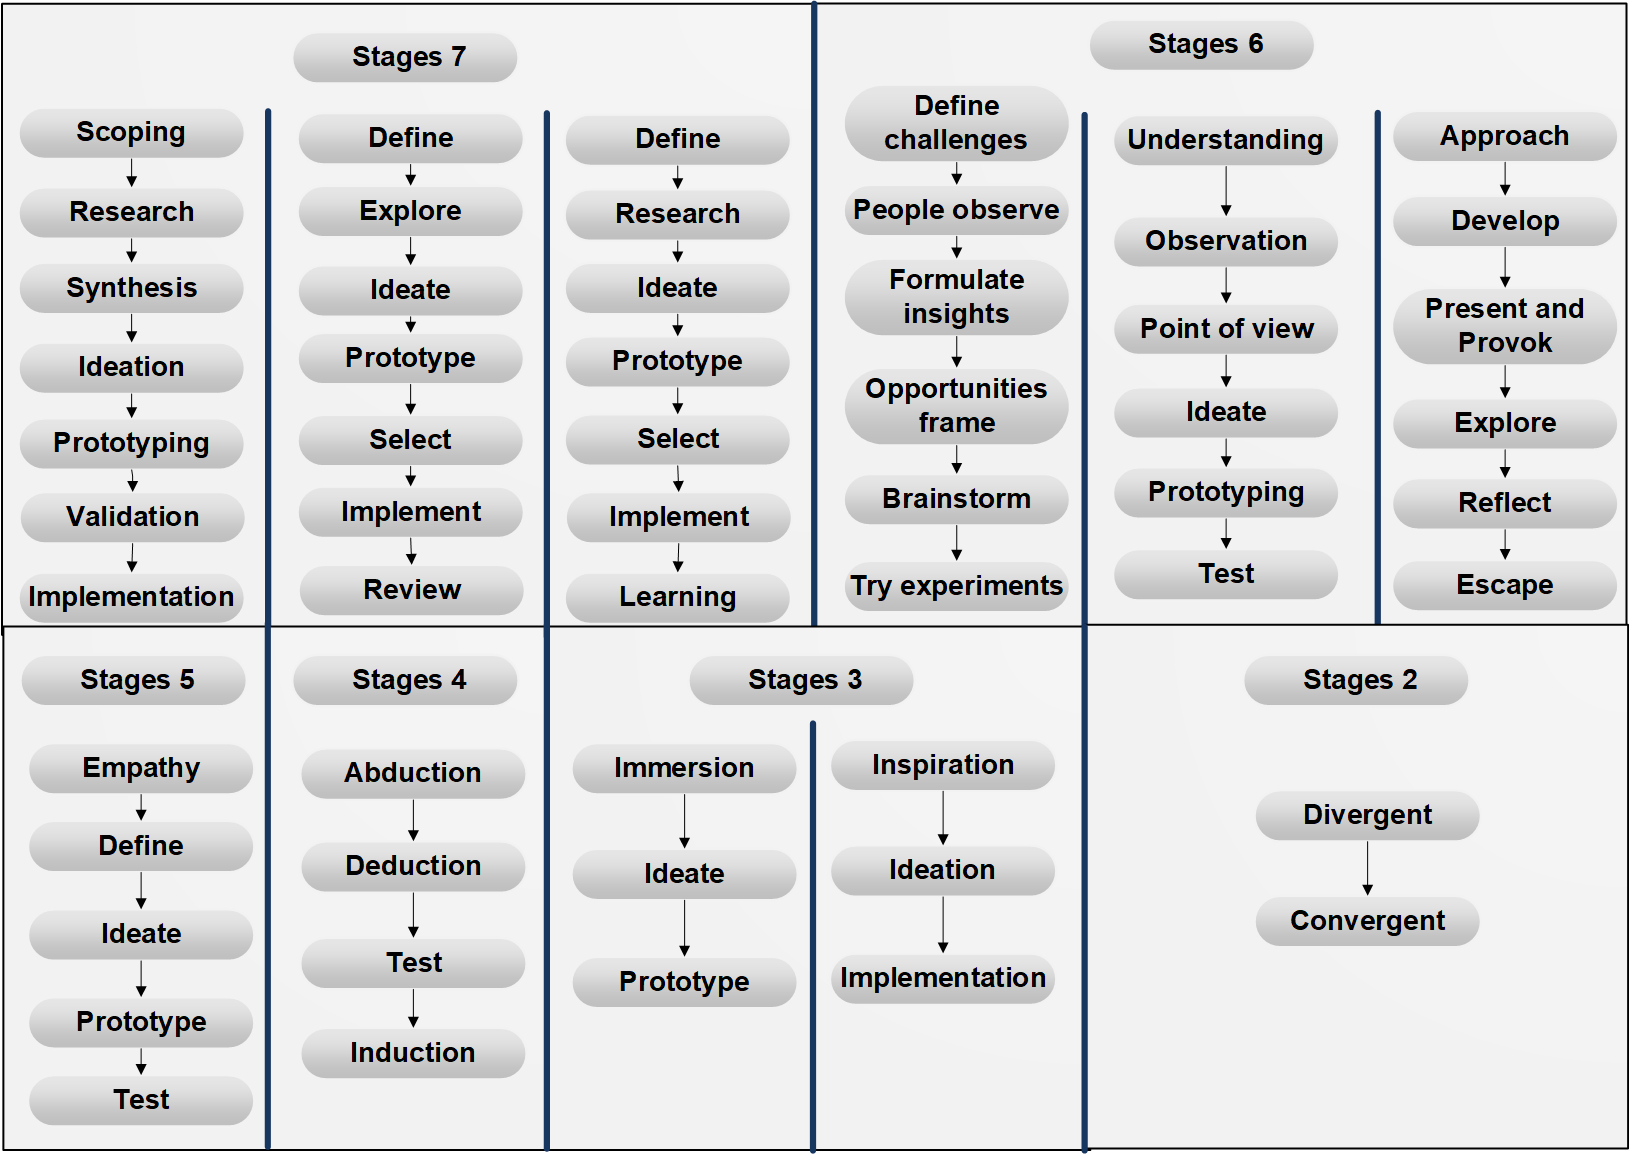
\includegraphics[width=3.2in]{Figures/ModelStages.png}    \caption{Design Thinking Process Models and and its Stages \cite{DBLP:conf/hci/CanedoC18}}
    \label{fig:my_label}
\end{figure}

Embora existam diversos modelos com diferentes fases, neste trabalho nós iremos considerar o modelo de 05 fases \cite{DBLP:conf/hci/XimenesAA15, DBLP:conf/icse/CarrollR16}.  

Algumas ferramentas de apoio ao Design Thinking na fase de elicitação de requisitos são:

Smaply: ferramenta de persona e outros métodos tais como
stakeholder map e customer journey maps
(http://www.smaply.com).
• Stakeholder Circle: ferramenta de stakeholder maps
(http://www.stakeholder-management.com/).
• Touchpoint Dashcboard: ferramenta de customer journey maps
(http://www.touchpointdashboard.com).
• Creately: ferramenta de service blueprint
(http://www.creately.com).
• Strategyzer: ferramenta de business model innovation
(http://www.strategyzer.com).
• Axure RP: ferramenta de prototipação rápida (http://
www.axure.com/)


\subsection{Requisitos de Privacidade}
\cite{DBLP:conf/wer/2019}
\subsection{Trabalhos Correlatos}

\todo[inline]{Aqui descrever os trabalhos que utilizam a empatia na elicitação de requisitos}

\section{Study Settings}
\label{method}

In this section we describe the settings of our study. We first state the goal of our investigation, and then we present details about the research questions we address and the procedures we take to conduct the study and collect issues from privacy requirements elicitation.

\subsection{Research Goal}

The main goal of this research is identificar na literatura e na indústria como a fase de Empatia do Design Thinking pode ser utilizada como ferramenta facilitadora na elicitação dos requisitos de privacidade. Neste trabalho, o nosso foco é em projetos de desenvolvimento de software. 

\subsection{Research Questions}
\label{rq}  

We conduct a multi-method study to investigate the following research questions:

\begin{enumerate}[RQ.1:]
    \item Como a fase de Empatia do Design Thinking pode motivar o desenvolvedor de software a identificar e tratar de forma eficaz os requisitos de privacidade?
    \item Quais as ferramentas relacionadas à fase de Empatia podem ser utilizadas para facilitar a elicitação de requisitos de privacidade? 
    \item A Empatia está relacionada a uma habilidade do desenvolvedor de software ou a uma orientação organizacional (processo padronizado/definido pela organização)?

\end{enumerate}

Para responder a RQ.1 e RQ.3 nós realizamos um grupo focal com os desenvolvedores de software da polícia militar do distrito federal PMDF. Nós exploramos questões relacionadas a .......

Para responder a RQ.2 nós realizamos uma revisão de literatura para identificar as ferramentas que são utilizadas na fase de Empatia na elicitação de requisitos e quais dessas ferramentas podem facilitar a elicitação de requisitos de privacidade.

\subsection{Research Methods}

\todo[inline]{aqui descreveremos rapidamente como foi configurado o grupo focal}

\section{STUDY RESULTS}
\label{empathy}

\subsection{Empathy and Privacy Rrquirements}

\todo[inline]{responder a questão de pesquisa : RQ.2 e sempre referenciar as afirmações}

\subsection{Focal Group}

\todo[inline]{aqui descreveremos os resultados com o grupo focal}

%
%\begin{figure*}[!t]
%\centering
%\subfloat[Case I]{\includegraphics[width=2.5in]{box}%
%\label{fig_first_case}}
%\hfil
%\subfloat[Case II]{\includegraphics[width=2.5in]{box}%
%\label{fig_second_case}}
%\caption{Simulation results for the network.}
%\label{fig_sim}
%\end{figure*}
%

%\begin{table}[!t]
%% increase table row spacing, adjust to taste
%\renewcommand{\arraystretch}{1.3}
% if using array.sty, it might be a good idea to tweak the value of
% \extrarowheight as needed to properly center the text within the cells
%\caption{An Example of a Table}
%\label{table_example}
%\centering
%% Some packages, such as MDW tools, offer better commands for making tables
%% than the plain LaTeX2e tabular which is used here.
%\begin{tabular}{|c||c|}
%\hline
%One & Two\\
%\hline
%Three & Four\\
%\hline
%\end{tabular}
%\end{table}


\section{Threats to Validity}
\label{thread}

\todo[inline]{Aqui descrever as ameaças para validação da pesquisa -- ver modelos outros artigos, falar sobre as ameaças a condução da revisão de literatura, ao grupo focal e etc.}


\section{Conclusion}
\label{conclusion}

\section*{Acknowledgment}

\bibliographystyle{IEEEtran}
\bibliography{paper}

\end{document}


